\iffalse
\title{PH:2015}
\author{AI24BTECH11007}
\section{ph}
\chapter{2015}
\fi
                          
	\item
		In the given circuit, the voltage across the source resistor is $1 \, V$. The drain voltage (in $V$) is \rule{2cm}{0.4pt}

		\hfill{(PH:2015)}
		\begin{center}
			
\begin{circuitikz}
    % Define the nodes and draw the circuit
    \draw
    % MOSFET transistor with labels
    (0,0) node[nmos, anchor=S] (M) {}

    % Source resistor to ground
    (M.S) -- ++(0,-1) 
    to[R=500~$\Omega$] ++(0,-1) node[ground]{}

    % Gate resistor to ground
    (M.G) -- ++(-1,0) 
    to[R=2~M$\Omega$] ++(0,-2) node[ground]{}

    % Drain resistor to power supply
    (M.D) -- ++(0,1) 
    to[R=5~k$\Omega$] ++(0,1) 
    -- ++(0,0.5) node[vsource, rotate=0] {25 V};

    % Draw a large circle around the NMOS transistor
    \draw[thick] (M) circle (1cm); % Adjust the radius as needed
    
    % Draw a small circle at the other end of the 5 kΩ resistor (connected to the voltage source)
    \draw[thick] ++(0, 3.7) circle (0.15cm); % Small circle at the top end of the 5 kΩ resistor

\end{circuitikz}


		\end{center}
		\vspace{0.5cm}
	\item
		A point charge is placed between two semi-infinite conducting plates which are inclined at an angle of $30\degree$ with respect to each other. The number of image charges is  \rule{2.5cm}{0.4pt}

		\hfill{(PH:2015)}
		\vspace{0.5cm}
	\item 
		A beam of X-ray of intensity $I_0$ is incident normally on a metal sheet of thickness $2 \, mm$. The intensity of the transmitted beam is $0.025I_0$. The linear absorption coefficient of the metal sheet (in $m^{-1}$) is \rule{2.5cm}{0.4pt} (upto one decimal place)

		\hfill{(PH:2015)}
		\vspace{0.5cm}
		\item
			The lattice parameters $a$, $b$, $c$ of an orthorhombic crystal are related by $a=\, 2b= \, 3c$. In units of $a$, the interplanar separation between the $(110)$ planes is \rule{2cm}{0.4pt} (upto three decimal places)

			\hfill{(PH:2015)}
			\vspace{0.5cm}
		\item
			In a Hall effect experiment, the Hall voltage for an intrinsic semiconductor is negative. This is because (symbols carry usual meaning)

			\hfill{(PH:2015)}
		\begin{multicols}{4}
			\begin{enumerate}
				\item $n\approx p$
				\item $n > p$
				\item $\mu_e > \mu_h$
				\item ${m_e}^* > {m_h}^*$
			\end{enumerate}
		\end{multicols}
	\item
		The space between two plates of a capacitor carrying charges $+Q$ and $-Q$ is filled with two different dielectric materials, as shown in figure. Across the interface of the two dielectric materials, which one of the following statements is correct?
		\begin{center}
			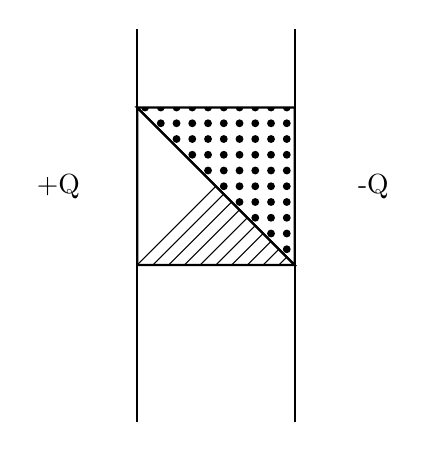
\begin{tikzpicture}
    % Draw the two parallel lines
    \draw[thick] (0,0) -- (0,5);
    \draw[thick] (2,0) -- (2,5);

    % Shaded area
   \begin{scope}
    % Clip to the first triangle
    \clip (0,2) -- (0,4) -- (2,2) -- cycle;
    % Draw diagonal lines
    \foreach \x in {-1, -0.8, ..., 3} { % Adjust range and spacing as needed
        \draw[thin] (\x,1) -- (\x+3,4); % Adjust angle and coverage
    }
\end{scope}
% Outline the first triangle
\draw[thick] (0,2) -- (0,4) -- (2,2) -- cycle;

% Second triangle with manual dots
\begin{scope}
    % Clip to the second triangle
    \clip (0,4) -- (2,2) -- (2,4) -- cycle;
    % Add dots manually using a foreach loop
    \foreach \x in {0.1,0.3,...,2.5} { % Adjust step size for spacing
        \foreach \y in {2.2,2.4,...,4.1} { % Adjust step size for density
            \fill (\x,\y) circle (0.05); % Adjust dot size
        }
    }
\end{scope}
% Outline the second triangle
\draw[thick] (0,4) -- (2,2) -- (2,4) -- cycle;
    % Labels
    \node at (-1,3) {+Q};
    \node at (3,3) {-Q};
\end{tikzpicture}

		\end{center}

		\hfill{(PH:2015)}
		\vspace{0.5cm}
	\begin{multicols}{2}
			\begin{enumerate}
				\item $\overrightarrow{E}$ and $\overrightarrow{D}$ are continuous
				\item $\overrightarrow{E}$ is continuous and $\overrightarrow{D}$ is discontinuous
				\item $\overrightarrow{D}$ is continuous and $\overrightarrow{E}$ is discontinuous
				\item $\overrightarrow{E}$ and $\overrightarrow{D}$ are discontinuous
			\end{enumerate}
		\end{multicols}
	\item 
		The energy dependence of the density of states for a two dimensional non-relativistic electron gas is given by, $g(E) = CE^n$, where $C$ is constant. The value of $n$ is \rule{2.5cm}{0.4pt}

		\hfill{(PH:2015)}
		\vspace{0.5cm}
	\item
		The dispersion relation for phonons in a one-dimensional monatomic Bravais lattice with lattice spacing $a$ and consisting of ions of masses $M$ is given by, $\omega(k) = \sqrt{\frac{2C}{M} \left[ 1 - \cos(ka) \right]},$ where $\omega$ is the frequency of oscillation, $k$ is the wavevector, and $C$ is the spring constant. For the long wavelength modes $(\lambda \gg a)$, the ratio of the phase velocity to the group velocity is \rule{2cm}{0.4pt}

		\hfill{(PH:2015)}
		\vspace{0.5cm}
	\item
		Four forces are given below in Cartesian and spherical polar coordinates.
\begin{itemize}
    \item[(i)] $\vec{F}_1 = K \exp\left(-\frac{r^2}{R^2}\right) \hat{r}$
    \item[(ii)] $\vec{F}_2 = K ( x^3 \hat{y} - y^3 \hat{z} )$
    \item[(iii)] $\vec{F}_3 = K ( x^3 \hat{x} + y^3 \hat{y} )$
    \item[(iv)] $\vec{F}_4 = K \left( \frac{\hat{\phi}}{r} \right)$
\end{itemize}

where $K$ is a constant. Identify the correct option.

\hfill{(PH:2015)}

\begin{enumerate}
    \item (iii) and (iv) are conservative but (i) and (ii) are not
    \item (i) and (ii) are conservative but (iii) and (iv) are not
    \item (ii) and (iii) are conservative but (i) and (iv) are not
    \item (i) and (iii) are conservative but (ii) and (iv) are not
\end{enumerate}
\item 
	Consider a system of eight non-interacting, identical quantum particles of spin$-\frac{3}{2}$ in a one dimensional box of length $L$. The minimum excitation energy of the system, in units of $\frac{\pi^2 \hbar^2}{2mL^2}$ is \rule{2cm}{0.4pt}

	\hfill{(PH:2015)}
	\vspace{0.5cm}
\item
	The excitation wavelength of laser in a Raman effect experiment is $546 \, nm$, then the wavenumber of the anti-Stokes' line (in $cm^{-1}$) is \rule{2cm}{0.4pt}

	\hfill{(PH:2015)}
	\vspace{0.5cm}
\item
	The binding energy per molecule of NaCl (lattice parameter is $0.563\, nm$) is $7.95\, eV$. The repulsive term of the potential is of the form $\frac{K}{r^9}$, where $K$ is a constant. The value of the Madelung constant is \rule{2cm}{0.4pt} (upto three decimal places)\\
	(Electron charge $e=\, -1.6\times 10^{-19}\, C;\, \epsilon_0 =\, 8.854\times 10^{-12} \, C^2 N^{-1} m^{-2}$  )

	\hfill{(PH:2015)}
	\vspace{0.5cm}
\item
	Given that the Fermi energy of gold is $5.54\, eV$, the number density of electrons is\\
	\rule{2cm}{0.4pt} $\times 10^{28}\, m^{-3}$ (upto one decimal place)\\
	\vspace{0.5cm}
(Mass of electron$=\, 9.11\times 10^{-31} \, kg;h=\, 6.626\times 10^{-34}J\cdot s; 1\, eV= \, 1.6\times 10^{-19}\, J$)

	\hfill{(PH:2015)}




